% =========================================================================
% Figura: Pipeline metodológico en 5 etapas para el modelado de MRP1 (3 arriba, 2 abajo)
% Paleta de colores accesible Okabe-Ito (Configurations/01-Colors.sty)
% =========================================================================

\begin{figure}[htbp]
\centering
\resizebox{0.98\linewidth}{!}{%
\begin{tikzpicture}[
    font=\sffamily,
    >=Stealth,
    x=1cm, y=1cm,
    cardStep/.style={draw=cardBorder, fill=white, rounded corners=6pt, line width=0.8pt},
    badgeNum/.style={circle, font=\fontsize{8}{9}\selectfont\bfseries, text=white, inner sep=2pt, minimum size=0.48cm}
]

% =========================================================================
% CONTENEDOR PRINCIPAL
% =========================================================================
\draw[draw=cardBorder, fill=cardBorder!6, rounded corners=8pt, line width=0.8pt] 
    (-0.25, -0.25) rectangle (16.25, 10.35);

% =========================================================================
% FILA SUPERIOR: 3 CUADROS (PASOS 1, 2 Y 3) - Ancho 5.1 cm cada uno
% =========================================================================

% ----------------- PASO 1: RECEPTOR 8VUX -----------------
\draw[cardStep] (0.0, 5.35) rectangle (5.10, 10.10);
\node[badgeNum, fill=figBlue] at (0.35, 9.75) {1};
\node[anchor=west, font=\fontsize{8.5}{10}\selectfont\bfseries, text=darkText] at (0.65, 9.75) {
    Receptor 8VUX
};

% Imagen de la proteína 8VUX
\node[inner sep=0pt] at (2.55, 8.10) {
    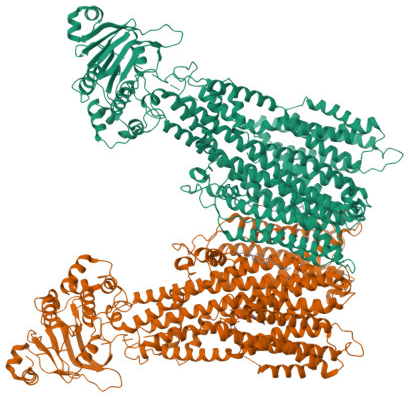
\includegraphics[height=2.20cm, width=4.75cm, keepaspectratio]{Figures/mrp1_estructura_cropped.png}
};

% Texto nítido y de alto contraste (2 líneas exactas)
\node[anchor=north, font=\fontsize{7.5}{9.4}\selectfont, text=darkText, align=center, text width=4.75cm] at (2.55, 6.75) {
    \textbf{Preparación de la Cadena B}\\[1.5pt]
    Limpieza y preparación estructural.
};

% Flecha 1 -> 2
\draw[line width=1.4pt, draw=figBlue, -{Stealth[length=5pt, width=4pt]}] 
    (5.15, 7.75) -- (5.45, 7.75);

% ----------------- PASO 2: BOLSILLO DE UNIÓN 78 -----------------
\draw[cardStep] (5.50, 5.35) rectangle (10.60, 10.10);
\node[badgeNum, fill=figOrange] at (5.85, 9.75) {2};
\node[anchor=west, font=\fontsize{8.5}{10}\selectfont\bfseries, text=darkText] at (6.15, 9.75) {
    Bolsillo de Unión 78
};

% Imagen de la cavidad (tutor_cavidad.png)
\node[inner sep=0pt, rounded corners=3pt] at (8.05, 8.10) {
    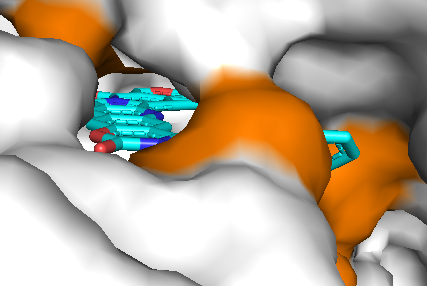
\includegraphics[height=2.20cm, width=4.75cm, keepaspectratio]{Figures/tutor_cavidad.png}
};

% Texto nítido y de alto contraste (2 líneas exactas)
\node[anchor=north, font=\fontsize{7.5}{9.4}\selectfont, text=darkText, align=center, text width=4.75cm] at (8.05, 6.75) {
    \textbf{Cavidad activa en TMD2}\\[1.5pt]
    Bolsillo 78 detectado con fpocket.
};

% Flecha 2 -> 3
\draw[line width=1.4pt, draw=figOrange, -{Stealth[length=5pt, width=4pt]}] 
    (10.65, 7.75) -- (10.95, 7.75);

% ----------------- PASO 3: CALIBRACIÓN CON IRINOTECÁN -----------------
\draw[cardStep] (11.0, 5.35) rectangle (16.10, 10.10);
\node[badgeNum, fill=figVermilion] at (11.35, 9.75) {3};
\node[anchor=west, font=\fontsize{8.5}{10}\selectfont\bfseries, text=darkText] at (11.65, 9.75) {
    Calibración (Irinotecán)
};

% Esquema conceptual y genérico: Irinotecán en la cavidad
\begin{scope}[shift={(13.55, 8.20)}]
    % Cavidad receptora (silueta suave en verde)
    \filldraw[draw=figGreen!80!black, fill=figGreenTint, line width=0.85pt]
        plot[smooth cycle, tension=0.6] coordinates {
            (-1.55, 0.75) (-0.20, 0.85) (1.20, 0.70) (1.65, 0.10) (1.35, -0.65) (0.00, -0.85) (-1.35, -0.70) (-1.70, -0.10)
        };

    % Ligando Irinotecán en el interior (centrado y limpio)
    \node[draw=figVermilion, fill=white, rounded corners=3pt, line width=0.8pt, font=\fontsize{7.5}{9}\selectfont\bfseries, text=darkText, inner sep=3.5pt] 
        (IRIN) at (0.0, 0.0) {Irinotecán};

    % Contactos en el sitio activo
    \coordinate (C1) at (-1.15, 0.50);
    \coordinate (C2) at (0.95, 0.50);
    \coordinate (C3) at (-1.00, -0.45);
    \coordinate (C4) at (1.00, -0.45);

    \draw[dashed, line width=0.8pt, draw=figOrange] (IRIN) -- (C1);
    \draw[dashed, line width=0.8pt, draw=figOrange] (IRIN) -- (C2);
    \draw[dashed, line width=0.8pt, draw=figOrange] (IRIN) -- (C3);
    \draw[dashed, line width=0.8pt, draw=figOrange] (IRIN) -- (C4);

    \filldraw[draw=darkText, fill=figOrange, line width=0.5pt] (C1) circle (0.10cm);
    \filldraw[draw=darkText, fill=figOrange, line width=0.5pt] (C2) circle (0.10cm);
    \filldraw[draw=darkText, fill=figOrange, line width=0.5pt] (C3) circle (0.10cm);
    \filldraw[draw=darkText, fill=figOrange, line width=0.5pt] (C4) circle (0.10cm);
\end{scope}

% Texto nítido y de alto contraste (2 líneas exactas)
\node[anchor=north, font=\fontsize{7.5}{9.4}\selectfont, text=darkText, align=center, text width=4.75cm] at (13.55, 6.75) {
    \textbf{Docking de calibración}\\[1.5pt]
    Simulación con ligando de referencia.
};

% =========================================================================
% FLECHA CONECTORA ENTRE FILAS (FLOTANTE, SIN COLISIONES)
% =========================================================================
\draw[line width=1.3pt, draw=grayText!70, -{Stealth[length=5.5pt, width=4pt]}] 
    (13.55, 5.35) -- (13.55, 4.92) -- (2.0, 4.92) -- (2.0, 4.50);

\node[fill=white, draw=cardBorder, rounded corners=2pt, inner sep=2pt, font=\fontsize{6.8}{8}\selectfont\bfseries, text=darkText] 
    at (7.80, 4.92) {Definición del espacio de búsqueda y evaluación de nuevos candidatos};

% =========================================================================
% FILA INFERIOR: 2 CUADROS (PASOS 4 Y 5) - Ancho 7.85 cm cada uno
% =========================================================================

% ----------------- PASO 4: DELIMITACIÓN DE LA CAJA DE DOCKING -----------------
\draw[cardStep] (0.0, 0.0) rectangle (7.85, 4.50);
\node[badgeNum, fill=figGreen] at (0.35, 4.15) {4};
\node[anchor=west, font=\fontsize{8.5}{10}\selectfont\bfseries, text=darkText] at (0.68, 4.15) {
    Delimitación de la Caja de Docking
};

% Lado izquierdo: Estructura de la proteína con la caja delimitadora en TMD2
\begin{scope}[shift={(1.85, 2.35)}]
    % Imagen de la proteína completa
    \node[inner sep=0pt] at (0, 0) {
        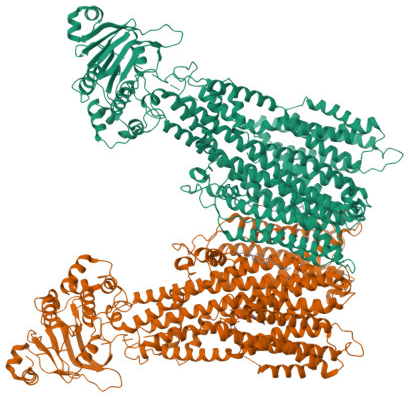
\includegraphics[height=2.40cm, width=3.30cm, keepaspectratio]{Figures/mrp1_estructura_cropped.png}
    };
    % Caja verde sobre el sitio de unión en TMD2
    \draw[draw=figGreen, fill=figGreenTint, fill opacity=0.35, line width=1.4pt, rounded corners=2pt] 
        (-0.85, -0.40) rectangle (0.85, 0.35);
    \node[circle, fill=figVermilion, inner sep=1.8pt] at (0.05, -0.05) {};
    \node[fill=figGreen, text=white, font=\fontsize{5.8}{6.8}\selectfont\bfseries, rounded corners=1.5pt, inner sep=1.5pt, anchor=north] 
        at (0.0, -0.42) {Caja $25\times 22\times 25\text{ \AA}$};
\end{scope}

% Lado derecho: Tarjeta de especificaciones técnicas con texto negro nítido
\begin{scope}[shift={(5.65, 2.45)}]
    \node[draw=cardBorder!70, fill=cardBorder!15, rounded corners=3pt, line width=0.6pt, minimum width=3.85cm, minimum height=1.95cm] at (0, 0) {};
    \node[anchor=north west, font=\fontsize{7.6}{10.2}\selectfont, text=darkText, align=left, text width=3.75cm] at (-1.82, 0.85) {
        \textbf{Caja de Búsqueda 3D:}\\[3pt]
        $\bullet$ \textbf{Dimensiones:} $25 \times 22 \times 25\text{ \AA}$\\[2.5pt]
        $\bullet$ \textbf{Centro:} $(166,\ 125,\ 124)\text{ \AA}$\\[2.5pt]
        $\bullet$ \textbf{Región:} TMD2 (Bolsillo 78)
    };
\end{scope}

% Texto explicativo inferior
\node[anchor=north, font=\fontsize{7.2}{8.8}\selectfont, text=darkText, align=center, text width=7.45cm] at (3.92, 0.55) {
    Volumen de búsqueda ajustado a la cavidad activa de MRP1.
};

% Flecha 4 -> 5
\draw[line width=1.4pt, draw=figGreen, -{Stealth[length=5pt, width=4pt]}] 
    (7.90, 2.25) -- (8.20, 2.25);

% ----------------- PASO 5: EVALUACIÓN DE CANDIDATOS -----------------
\draw[cardStep] (8.25, 0.0) rectangle (16.10, 4.50);
\node[badgeNum, fill=figGreen] at (8.60, 4.15) {5};
\node[anchor=west, font=\fontsize{8.5}{10}\selectfont\bfseries, text=darkText] at (8.93, 4.15) {
    Evaluación de Candidatos
};

% Esquema adaptado directamente de la figura de Docking del Marco Teórico (docking_molecular.tex)
\begin{scope}[shift={(12.175, 2.65)}]
    % Izquierda: Ligando candidato (representación ball-and-stick de docking_molecular.tex)
    \begin{scope}[shift={(-2.15, 0.05)}]
        \coordinate (L_c) at (0.0, 0.0);
        \coordinate (L_1) at (-0.40, 0.10);
        \coordinate (L_2) at (-0.20, 0.55);
        \coordinate (L_3) at (0.40, 0.20);
        \coordinate (L_4) at (-0.20, -0.55);
        \coordinate (L_5) at (0.30, -0.45);

        \draw[line width=1.0pt, draw=darkText] (L_c) -- (L_1);
        \draw[line width=1.0pt, draw=darkText] (L_c) -- (L_2);
        \draw[line width=1.0pt, draw=darkText] (L_c) -- (L_3);
        \draw[line width=1.0pt, draw=darkText] (L_c) -- (L_4);
        \draw[line width=1.0pt, draw=darkText] (L_c) -- (L_5);

        \filldraw[draw=darkText, fill=figOrangeTint, line width=0.7pt] (L_1) circle (0.10cm);
        \filldraw[draw=darkText, fill=figOrangeTint, line width=0.7pt] (L_2) circle (0.10cm);
        \filldraw[draw=darkText, fill=figOrangeTint, line width=0.7pt] (L_3) circle (0.10cm);
        \filldraw[draw=darkText, fill=figOrangeTint, line width=0.7pt] (L_4) circle (0.10cm);
        \filldraw[draw=darkText, fill=figOrangeTint, line width=0.7pt] (L_5) circle (0.10cm);
        \filldraw[draw=darkText, fill=figOrange, line width=0.8pt] (L_c) circle (0.15cm);

        \node[font=\fontsize{6.8}{8}\selectfont\bfseries, text=darkText] at (0.0, -0.90) {Ligando candidato};
    \end{scope}

    % Centro: Flecha de acoplamiento por docking
    \draw[line width=1.4pt, draw=figGreen, -{Stealth[length=5.5pt, width=4pt]}] (-0.80, 0.05) -- (0.50, 0.05);
    \node[font=\fontsize{7.2}{8.5}\selectfont\bfseries, text=figGreen!90!black] at (-0.15, 0.35) {Docking};
    \node[font=\fontsize{6.2}{7.2}\selectfont, text=darkText!70] at (-0.15, -0.22) {Acoplamiento};

    % Derecha: Receptor con cavidad y ligando acoplado en el sitio activo (docking_molecular.tex)
    \begin{scope}[shift={(1.85, 0.05)}]
        % Receptor con proporción y cavidad original
        \filldraw[draw=figGreen!80!black, fill=figGreenTint, line width=0.85pt]
            plot[smooth cycle, tension=0.6] coordinates {
                (0.05, 0.85) (0.55, 0.65) (0.80, 0.20) (0.70, -0.25) (0.80, -0.65) (0.35, -0.95) (-0.25, -0.80) (-0.50, -0.35)
                (-0.05, -0.18) (0.00, 0.18) (-0.20, 0.40) (-0.55, 0.52) (-0.25, 0.85)
            };

        % Ligando acoplado en el sitio activo 
        \coordinate (S_c) at (-0.15, 0.05);
        \coordinate (S_1) at (-0.45, 0.28);
        \coordinate (S_2) at (0.15, 0.32);
        \coordinate (S_3) at (0.00, -0.28);
        \coordinate (S_4) at (-0.50, -0.10);

        \draw[line width=0.9pt, draw=darkText] (S_c) -- (S_1);
        \draw[line width=0.9pt, draw=darkText] (S_c) -- (S_2);
        \draw[line width=0.9pt, draw=darkText] (S_c) -- (S_3);
        \draw[line width=0.9pt, draw=darkText] (S_c) -- (S_4);

        \filldraw[draw=darkText, fill=figOrangeTint, line width=0.5pt] (S_1) circle (0.07cm);
        \filldraw[draw=darkText, fill=figOrangeTint, line width=0.5pt] (S_2) circle (0.07cm);
        \filldraw[draw=darkText, fill=figOrangeTint, line width=0.5pt] (S_3) circle (0.07cm);
        \filldraw[draw=darkText, fill=figOrangeTint, line width=0.5pt] (S_4) circle (0.07cm);
        \filldraw[draw=darkText, fill=figOrange, line width=0.6pt] (S_c) circle (0.10cm);

        \node[font=\fontsize{6.8}{8}\selectfont\bfseries, text=figGreen!90!black] at (0.10, -1.20) {Pose acoplada ($\Delta G$)};
    \end{scope}
\end{scope}

% Texto explicativo inferior nítido (2 líneas exactas con margen cómodo, sin "3D")
\node[anchor=north, font=\fontsize{7.5}{9.4}\selectfont, text=darkText, align=center, text width=6.80cm] at (12.175, 1.00) {
    \textbf{Evaluación de Candidatos}\\[1.5pt]
    Acoplamiento molecular y cálculo de afinidad de unión.
};

\end{tikzpicture}%
}
\caption{Flujo metodológico en cinco etapas para el modelado de MRP1: preparación del receptor, identificación del bolsillo de unión, calibración con ligando de referencia, delimitación de la caja de docking sobre la cavidad y evaluación de las moléculas candidatas mediante docking.}
\label{fig:pipeline_preparacion_mrp1}
\end{figure}
